\chapter{Umsetzung und Ergebnisse}
\label{chap:Umsetzung und Ergebnisse}
\section{Umsetzung}
\subsection{Einfache Echo-Nachricht}
Das Projekt begann ich mit der Datei \texttt{main.py}, die später zur Server-Datei wurde (siehe unten). Ihre Aufgabe bestand zunächst darin, sich mit einem Client zu verbinden und empfangene Nachrichten unverändert zurückzusenden. Dazu wird ein Socket an die IP-Adresse des Servers und den festgelegten Port 7367 gebunden. Mit \texttt{server.listen()} wartet der Socket auf Verbindungsanfragen, und \texttt{server.accept()} nimmt eine Anfrage an. Der zugrunde liegende Three-Way-Handshake wird dabei vom Betriebssystem durchgeführt. Mit \texttt{client.recv(1024)} empfängt der Server die Daten des Clients und sendet sie mit \texttt{client.sendall(data)} zurück. Die Methode \texttt{sendall()} wiederholt den Sendevorgang, bis alle Bytes übertragen sind. Bei \texttt{send()} kann es dagegen vorkommen, dass nur ein Teil der Daten gesendet wird.\\

\begin{figure}[H]
    \centering
    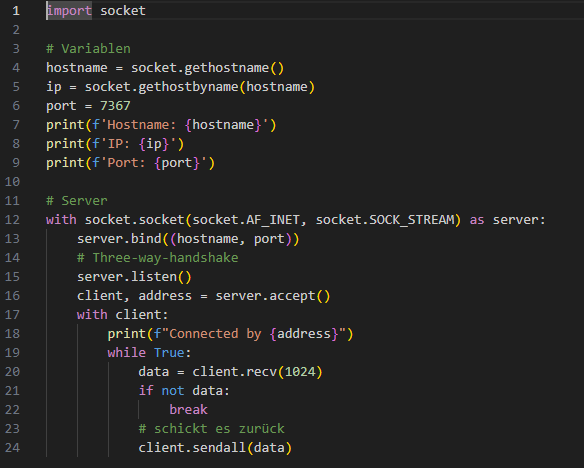
\includegraphics[width=0.5\linewidth]{picture-lib/Screenshot 2026-10-07 020521.png}
    \caption{Server.py V1}
    \label{fig:A0}
\end{figure}

Danach erstellte ich die Datei \texttt{client.py}, die der Benutzer benötigt, um mit dem Server zu kommunizieren. Sie verbindet sich mit der IP-Adresse des Servers und dem Port 7367 und sendet die Nachricht "Test" als Bytes. Anschliessend wartet sie auf die Antwort des Servers und wandelt die empfangenen Bytes wieder in eine Zeichenkette (String) um.\\

\begin{figure}[H]
    \centering
    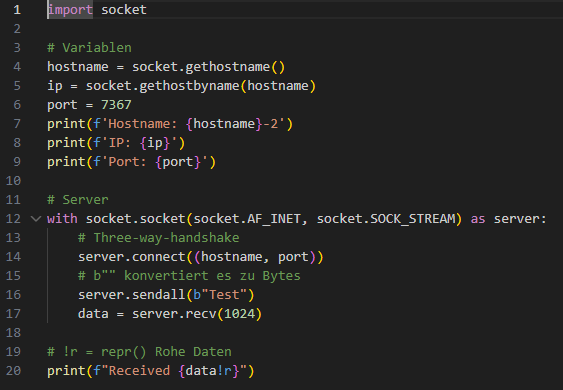
\includegraphics[width=0.5\linewidth]{picture-lib/Screenshot 2026-10-07 020618.png}
    \caption{Client.py V1}
    \label{fig:A1}
\end{figure}

Mit diesen beiden Dateien war ein erster Nachrichtenaustausch zwischen Server und Client möglich.

\subsection{Mehrere Benutzer}

Als Nächstes erweiterte ich den Server so, dass mehrere Clients gleichzeitig kommunizieren können, ohne aufeinander warten zu müssen. Der Server bindet sich wie zuvor an IP-Adresse und Port. Mit \texttt{server.listen(5)} legt er jedoch eine Warteschlange von höchstens fünf unbearbeiteten Verbindungsanfragen fest. Danach läuft eine while-Schleife, die jede eingehende Verbindung annimmt. Mit der Bibliothek Threading wird für jeden Client ein eigener Thread erstellt, der die Funktion \texttt{client\_handler(client)} ausführt. Innerhalb dieser Funktion läuft eine weitere while-Schleife, die auf eingehende Daten wartet. Sie wird beendet, wenn der Client die Verbindung trennt oder ein Fehler auftritt. Andernfalls sendet der Server die Daten in umgekehrter Reihenfolge zurück (\texttt{data[::-1]}).

\begin{figure}[H]
    \centering
    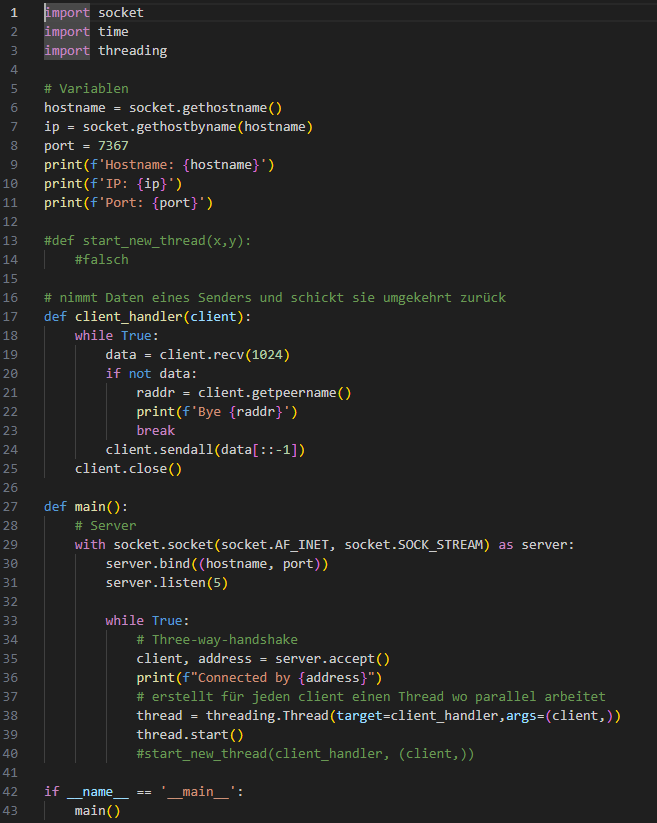
\includegraphics[width=0.5\linewidth]{picture-lib/Screenshot 2026-10-07 022627.png}
    \caption{Server.py V2}
    \label{fig:A2}
\end{figure}

Auch die Client-Datei wurde überarbeitet. Eine while-Schleife ermöglicht nun mehrere Nachrichten nacheinander. Zudem liest das Programm die Eingabe im Terminal mit \texttt{input()} und speichert sie in der Variable \texttt{message}. Diese wird mit der Zeichenkodierung ASCII in Bytes umgewandelt und gesendet. Die Antwort des Servers wird anschliessend mit ASCII dekodiert und dem Benutzer angezeigt. Am Ende jedes Durchlaufs fragt das Programm, ob der Benutzer fortfahren möchte. Bei der Eingabe "y" beginnt die Schleife von vorn, bei jeder anderen Eingabe wird die Verbindung getrennt.

\begin{figure}[H]
    \centering
    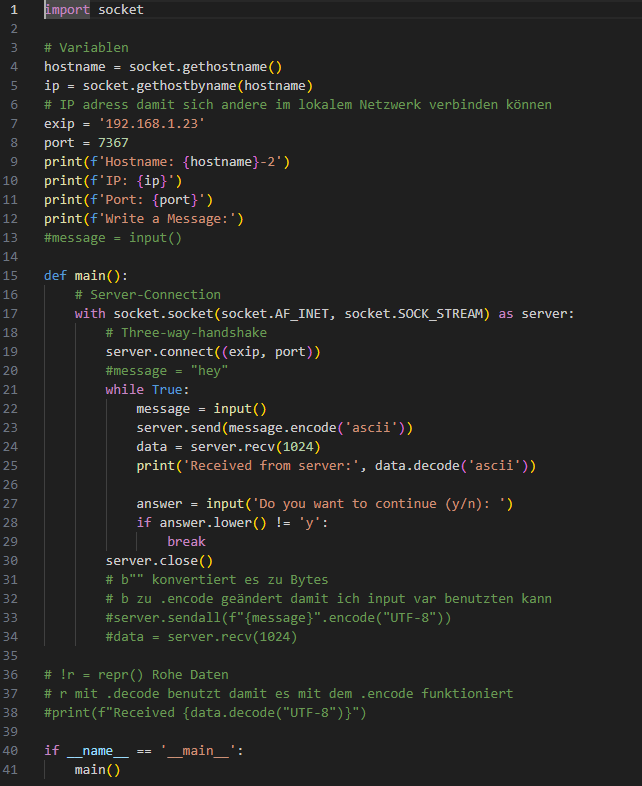
\includegraphics[width=0.5\linewidth]{picture-lib/Screenshot 2026-10-07 022613.png}
    \caption{Client.py V2}
    \label{fig:A3}
\end{figure}

Beide Dateien zusammen erlauben den Datenaustausch zwischen mehreren Clients und dem Server. Die Clients können in dieser Version nur mit dem Server Daten austauschen, untereinander ist keine Kommunikation möglich.

\subsection{Austausch von Informationen}

In der nächsten Version wurde die Kommunikation zwischen Benutzern ermöglicht. Der Server empfängt eine Nachricht von einem Client und leitet sie an den richtigen Empfänger weiter. Der Verbindungsaufbau blieb bis auf eine Ausnahme gleich: Es wird nun eine Liste \texttt{client\_connections} geführt, in die jeder verbundene Client eingetragen wird. Diese Liste wird an den \texttt{client\_handler} übergeben. Er wartet innerhalb eines \texttt{try}-Blocks auf Daten. Treten Fehler auf, bricht er den Vorgang ab, sendet eine Fehlermeldung, schliesst die Verbindung und entfernt den Client aus der Liste.
Treffen Daten ein, wird zwischen einer Nachricht und dem Befehl \texttt{GET\_LIST} unterschieden. Bei diesem Befehl sendet der Server dem Client die Liste aller aktuell verbundenen Clients, ohne den Anfragenden selbst. Das wird mit der Bedingung \texttt{if x != address} geprüft. Die übrigen Adressen werden in der Variable \texttt{users} gespeichert, mit \texttt{.join(users)} zu einer Zeichenkette verbunden, mit ASCII kodiert und gesendet.
Handelt es sich um eine Nachricht, prüft der Server zuerst die IP-Adresse des Empfängers mithilfe der Statusvariable \texttt{found} (Flag). Eine Schleife vergleicht dazu alle bestehenden Verbindungen mit der Empfängeradresse. Bei einer Übereinstimmung wird die Nachricht gesendet, \texttt{found} auf wahr gesetzt und die Schleife beendet. Existiert der Empfänger nicht oder ist er nicht mehr verbunden, bleibt \texttt{found} falsch, und \texttt{if not found:} meldet dem Absender, dass der Empfänger nicht gefunden wurde.

\begin{figure}[H]
    \centering
    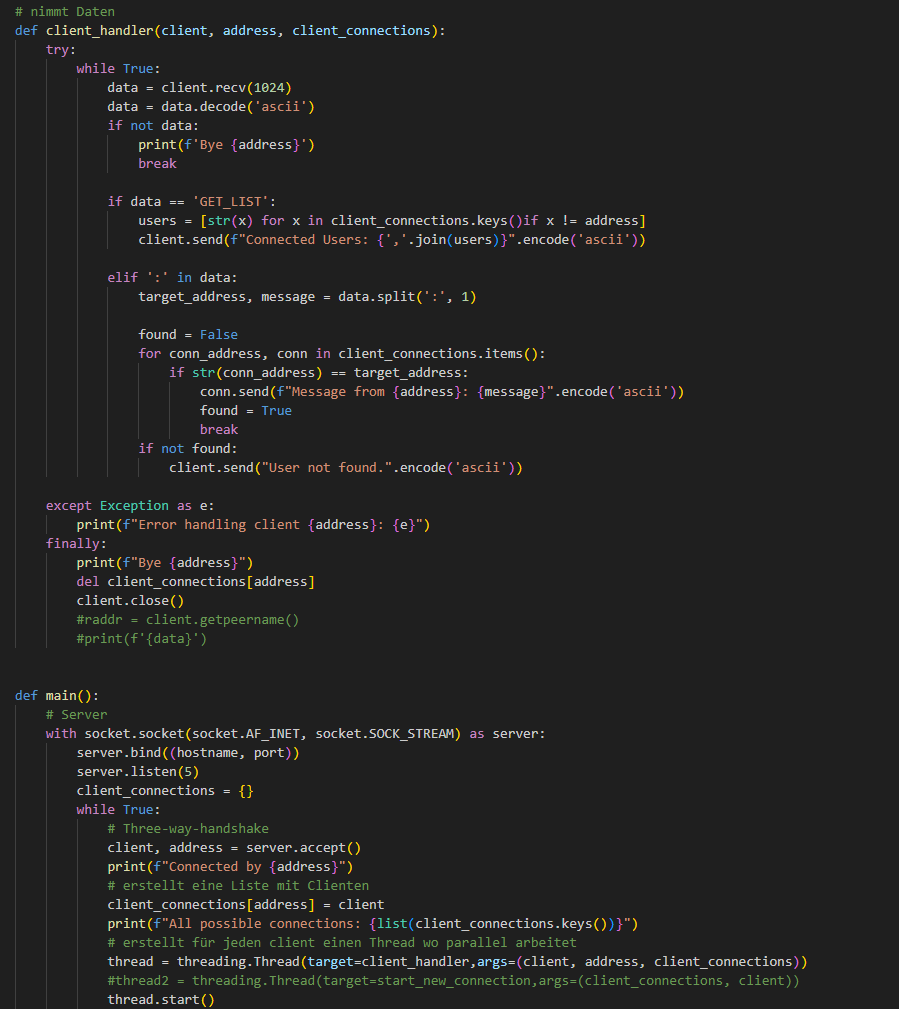
\includegraphics[width=0.5\linewidth]{picture-lib/Screenshot 2026-10-07 025514.png}
    \caption{Server.py V3}
    \label{fig:A4}
\end{figure}

In der Client-Datei wurde ein Daemon Thread ergänzt, damit die Eingabe des Benutzers nicht blockiert wird. Dieser führt die Funktion \texttt{receive\_messages(client\_data)} aus, die in einer Schleife auf Nachrichten wartet. Durch den Wert \texttt{daemon=True} läuft sie im Hintergrund, übersetzt alle ankommenden Daten mit ASCII und zeigt sie im Terminal an. Gleichzeitig läuft eine Schleife für die Eingabe, die bei jedem Durchlauf drei Fälle unterscheidet. Gibt der Benutzer \texttt{list} ein, sendet der Client den Befehl \texttt{GET\_LIST} an den Server. Bei \texttt{exit} wird die Schleife beendet. Jede andere Eingabe wird als Nachricht an den Server gesendet. In dieser Version muss der Benutzer IP-Adresse, Port und Nachricht selbst eingeben. Bei einer fehlerhaften Eingabe kommt die Nachricht nicht beim gewünschten Empfänger an.

\begin{figure}[H]
    \centering
    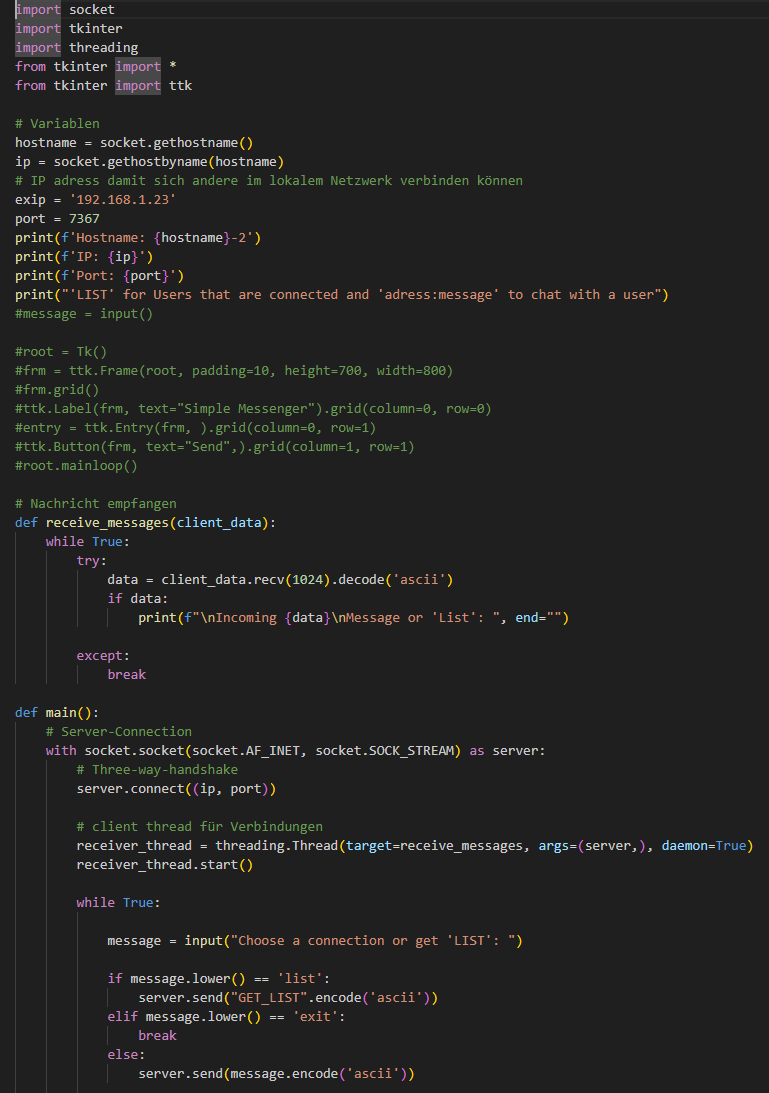
\includegraphics[width=0.5\linewidth]{picture-lib/Screenshot 2026-10-07 025429.png}
    \caption{Client.py V3}
    \label{fig:A5}
\end{figure}

Die beiden Dateien bilden ein Backend für die Kommunikation zwischen Benutzern, das allerdings wenig benutzerfreundlich ist. Der Server speichert die Adressen der Clients, filtert sie und leitet Nachrichten an den richtigen Empfänger weiter.

\subsection{GUI für Benutzer}

Bei der Programmierung der GUI blieb die Server-Datei fast unverändert und wird hier nicht weiter behandelt. Mit der Bibliothek Tkinter lässt sich ein Frontend, also eine grafische Benutzeroberfläche, erzeugen. Zuerst mussten empfangene Nachrichten im Fenster dargestellt werden. Das funktioniert nach demselben Prinzip wie in Version 3: Die Daten werden mit ASCII dekodiert, und wie in der Server-Datei wird zwischen Liste und Nachricht unterschieden. Das Unterscheidungsmerkmal für eine Nachricht ist der Doppelpunkt. Sie wird als \texttt{notification} gespeichert und im Fenster \texttt{chat\_box} angezeigt. Enthalten die Daten keinen Doppelpunkt, werden sie als Liste behandelt. Dabei werden die Klammern jeder Adresse entfernt, die Adressen in der Liste \texttt{user\_list} gespeichert und anschliessend als Werte der Combobox hinzugefügt.

\begin{figure}[H]
    \centering
    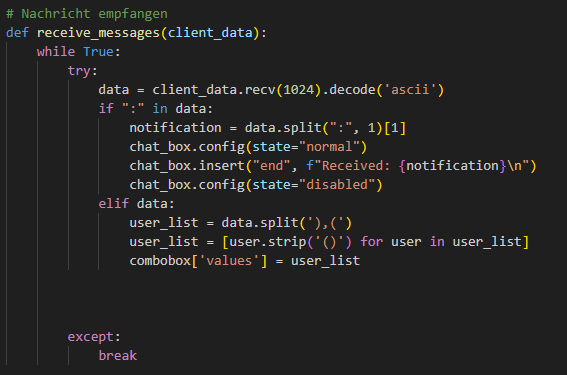
\includegraphics[width=0.5\linewidth]{picture-lib/Screenshot 2026-10-07 042912.png}
    \caption{Client.py V4 Abschnitt 1}
    \label{fig:A6}
\end{figure}

In der Hauptfunktion wird die GUI aufgebaut. Zuerst entsteht mit \texttt{tk.Tk()} das Fenster, das alle Widgets enthält. Anschliessend werden die Widgets Label, Text, Button, Combobox und Entry erstellt und in Variablen gespeichert. Wichtig sind die beiden Schaltflächen und das Eingabefeld. Die Schaltfläche "Get List" (\texttt{button2}) ruft die Funktion \texttt{get\_list()} auf, die dem Server den Befehl \texttt{GET\_LIST} sendet. Die Schaltfläche "Send" ruft die Funktion \texttt{send()} auf.

\begin{figure}[H]
    \centering
    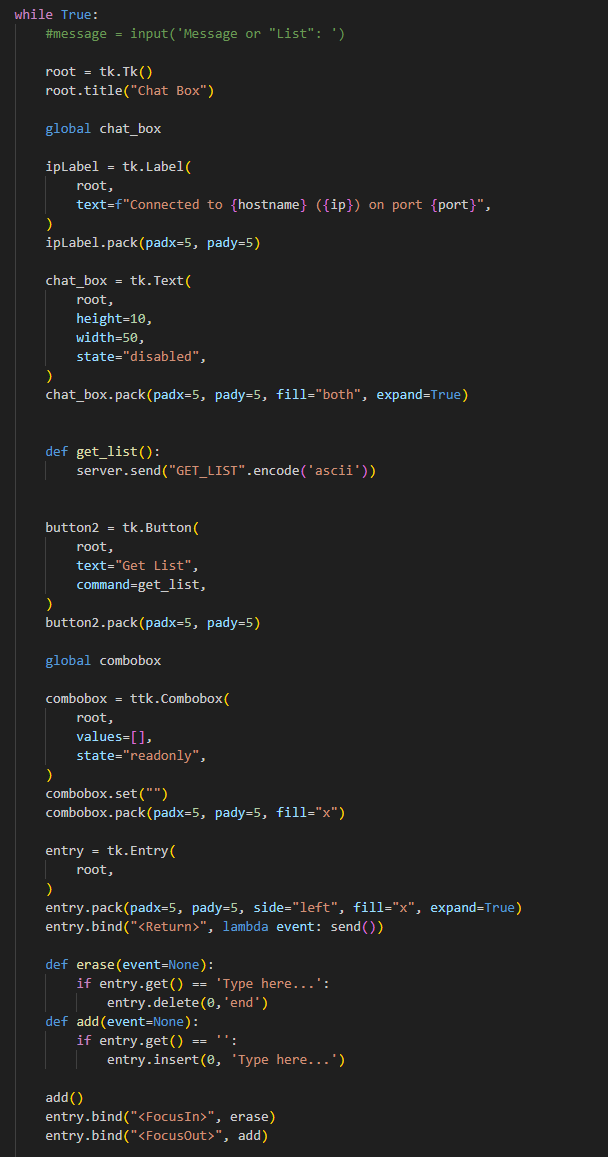
\includegraphics[width=0.45\linewidth]{picture-lib/Screenshot 2026-10-07 042949.png}
    \caption{Client.py V4 Abschnitt 2}
    \label{fig:A7}
\end{figure}

Die Funktion \texttt{send()} übernimmt mehrere Aufgaben. Zuerst liest sie die vom Benutzer in der Combobox ausgewählte Adresse und kombiniert sie mit dem Text aus dem Eingabefeld zur Variable \texttt{message}. Danach sendet sie die Nachricht an den Server und zeigt im Chatverlauf an, welche Nachricht an wen gesendet wurde. Anschliessend leert sie das Eingabefeld und verändert den Fensterfokus, damit der Platzhalter "Type here\dots" wieder erscheint. Beim Schreiben verschwindet er erneut. Beim Schliessen des Fensters erscheint eine Sicherheitsabfrage. Bestätigt der Benutzer mit "Yes", werden das Fenster und die Verbindung geschlossen, damit das Programm nicht im Hintergrund weiterläuft.

\begin{figure}[H]
    \centering
    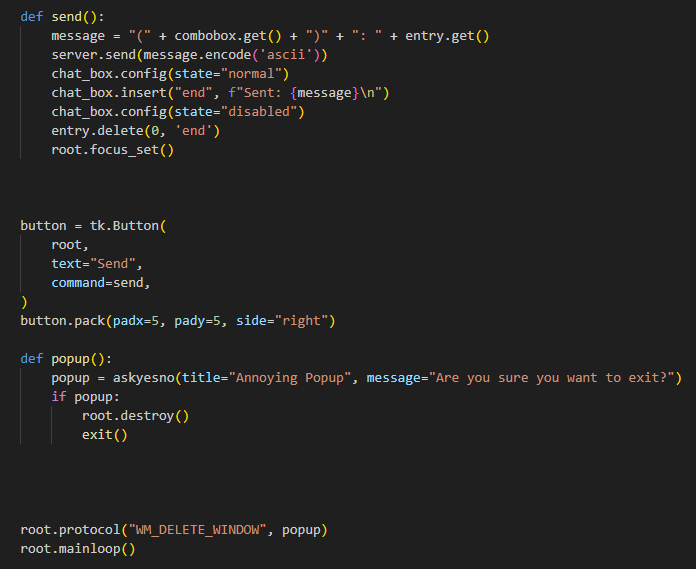
\includegraphics[width=0.5\linewidth]{picture-lib/Screenshot 2026-10-07 043004.png}
    \caption{Client.py V4 Abschnitt 3}
    \label{fig:A8}
\end{figure}

Daraus ergibt sich die Chat Box in der Abbildung \ref{fig:A9}.

\begin{figure}[H]
    \centering
    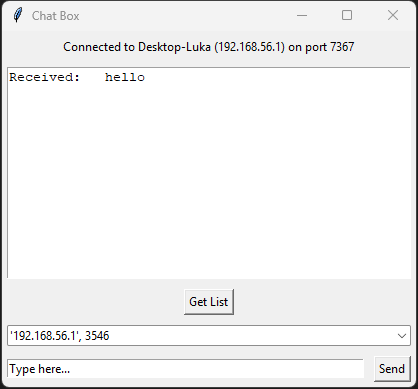
\includegraphics[width=0.5\linewidth]{picture-lib/Screenshot 2026-10-07 045701.png}
    \caption{Chat Box}
    \label{fig:A9}
\end{figure}

Über diese Oberfläche kann der Benutzer einen aktuell mit dem Server verbundenen Teilnehmer auswählen und ihm Nachrichten senden sowie selbst Nachrichten empfangen. Alle Nachrichten erscheinen im Chatverlauf.

\subsection{Verschlüsselung und separates Protokoll}

In der separaten Datei \texttt{test.py} experimentierte ich, bis ich die Verschlüsselung verstanden hatte, und entwickelte ein eigenes Protokoll, das innerhalb des bestehenden Socket-Protokolls arbeitet. Die Sockets selbst lassen sich kaum verändern, und Methoden ohne Sockets werden vom Schulnetzwerk gesperrt. Deshalb kann ich nur die über die Sockets übertragenen Daten beeinflussen.
Aus der Bibliothek Pycryptodomex importierte ich AES, womit sich Bytes ver- und entschlüsseln lassen. Zuerst erstellte ich eine Beispielnachricht und wandelte sie in Bytes um. Als Testschlüssel wählte ich die 16 Byte lange Zeichenkette "Sixteen byte key", die ebenfalls in Bytes umgewandelt wird. Um den Code im eigentlichen Projekt wiederzuverwenden, definierte ich die Funktion \texttt{cipher\_message(message, key)}. Sie erhält die Nachricht als String und den Schlüssel als Bytes. Bei jedem Aufruf wird eine neue Verschlüsselung mit \texttt{AES.new(key, AES.MODE\_EAX)} im EAX-Modus (Encrypt-then-Authenticate-then-Translate) erzeugt.\citep{EAXModus2021} EAX verschlüsselt und authentifiziert die Nachricht. Wird sie auf dem Weg manipuliert, meldet der Empfänger mit dem richtigen Schlüssel dies bei der Prüfung.
Für die Verschlüsselung wird ausserdem ein Nonce (number used once) erzeugt, eine zufällige Zahl, die mit den Daten und dem Schlüssel verknüpft wird. Der Nonce darf öffentlich bekannt sein, darf sich aber bei demselben Schlüssel nie wiederholen, da sonst die Sicherheit der Verschlüsselung verloren geht. Anschliessend wird die Nachricht mit \texttt{cipher.encrypt\_and\_digest()} verschlüsselt. Innerhalb der Klammer wird der String mit UTF-8 in Bytes umgewandelt, da UTF-8 auch Sonderzeichen wie ä, ö und ü unterstützt. Zusätzlich liefert EAX einen Tag, der zur Validierung dient. Die Funktion gibt Tag, Nonce und verschlüsselten Text zurück.

\begin{figure}[H]
    \centering
    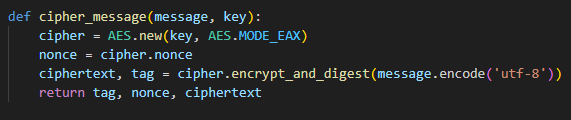
\includegraphics[width=0.75\linewidth]{picture-lib/Screenshot 2026-10-07 194013.png}
    \caption{Test.py Abschnitt 1}
    \label{fig:A10}
\end{figure}

Danach plante ich den Aufbau eines eigenen Protokolls. Ich skizzierte es zuerst auf Papier und stelle es hier als Tabelle \ref{tab:T1} dar.

\begin{table}[H]
    \centering
    \begin{tabular}{|c|c|c|c|c|c|}\hline
          Indikator&  IP&  Port&  Tag&  Nonce& Kryptogramm\\\hline
  [0x0], [0x1] oder [0x2]& 192.168.1.x& 7376& Prüfsumme& Zufällige Zahl&Vermischte Bytes\\ \hline 
    \end{tabular}
    \caption{Eigenes Protokoll}
    \label{tab:T1}
\end{table}

Anschliessend setzte ich es in der Funktion \texttt{construct\_message(\dots)} um. Sie erhält IP-Adresse, Port, Tag, Nonce und Kryptogramm und fügt sie zu einem eigenen Datenpaket zusammen. Zuerst werden IP-Adresse (String) und Port (Integer) mit der Bibliothek Socket in Bytes umgewandelt. Danach wird das Datenpaket in der Reihenfolge der Tabelle aufgebaut. Da es sich um eine Nachricht handelt, ist das erste Byte der Indikator [0x1].

\begin{figure}[H]
    \centering
    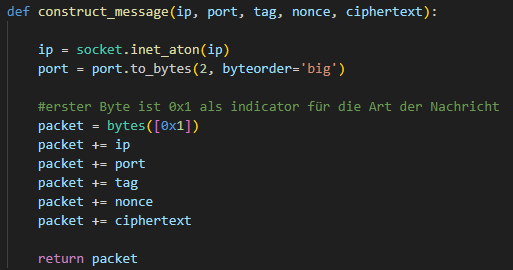
\includegraphics[width=0.5\linewidth]{picture-lib/Screenshot 2026-10-07 194028.png}
    \caption{Test.py Abschnitt 2}
    \label{fig:A11}
\end{figure}

Zuletzt definierte ich die Umkehrfunktion \texttt{decipher\_message(\dots)}. Sie benötigt denselben Schlüssel wie der Sender sowie Tag und Nonce. Mit Nonce und Schlüssel erzeugt sie dasselbe Verschlüsselungsobjekt wie der Sender. Das Kryptogramm wird mit \texttt{cipher.decrypt()} entschlüsselt und liegt danach als Klartext in Bytes vor. Mit \texttt{cipher.verify(tag)} wird die Gültigkeit geprüft. Ist sie gegeben, gibt die Funktion die Nachricht zurück, andernfalls eine Fehlermeldung.

\begin{figure}[H]
    \centering
    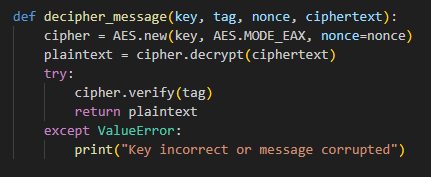
\includegraphics[width=0.5\linewidth]{picture-lib/Screenshot 2026-10-07 193959.png}
    \caption{Test.py Abschnitt 3}
    \label{fig:A12}
\end{figure}

Diese drei Funktionen ermöglichen den Austausch verschlüsselter Nachrichten in einem Netzwerk. Zudem lässt sich damit prüfen, ob die Daten auf dem Weg zum Empfänger verändert oder beschädigt wurden.

\section{Ergebnisse}

\subsection{Serverseite}

Zu Beginn werden die wichtigen Variablen des Servers festgelegt. Dazu gehört ein Puffer (Buffer) von 4 KB, was bei ASCII-Zeichen etwa 4000 Zeichen entspricht und für Textnachrichten ausreicht. Danach folgen IP-Adresse und Port. Beim Server muss die IP-Adresse 0.0.0.0 lauten, damit er auf allen Netzwerkschnittstellen Verbindungen annimmt, und der Port darf nicht bereits belegt sein. Der gewählte Port ist allerdings schon von der Swiss Exchange belegt, was bei Geräten, die diese Verbindung offen haben, zu Konflikten führen könnte.\todo{Quelle für die Port-Belegung ergänzen} Das war mir bis zu diesem Zeitpunkt nicht bekannt, da ich die Zahl zufällig gewählt und nicht überprüft hatte.

\begin{figure}[H]
    \centering
    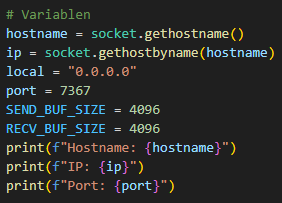
\includegraphics[width=0.5\linewidth]{picture-lib/Screenshot 2026-10-07 205017.png}
    \caption{Server.py Finale Version Abschnitt 1}
    \label{fig:A13}
\end{figure}

In der finalen Version mussten einige Funktionen angepasst werden, damit sie mit meinem Protokoll arbeiten. Der Server liest zuerst das erste Byte des Datenpakets, den Indikator, und unterscheidet damit zwischen Listenbefehl und Nachricht. Ist das erste Byte 0x0, baut er eine Liste der bestehenden Verbindungen auf, diesmal im Byte-Format. Auch diese Liste beginnt mit 0x0, damit sie als Liste erkannt wird. Für jeden Benutzer werden IP-Adresse und Port als Bytes angehängt. Das geschieht in einer for-Schleife, die alle Benutzer ausser dem anfragenden durchläuft.
Ist der Indikator 0x1, erkennt der Server eine Nachricht und liest IP-Adresse und Port des Empfängers. Stimmen sie mit einer bestehenden Verbindung überein, sendet er die Nachricht an diese Verbindung. Wird der Empfänger nicht gefunden, zeigt der Server dies an und sendet dem Absender ein Byte 0x2 als Fehlercode. Der Server liest dabei nur die ersten drei Felder des Protokolls (Indikator, IP-Adresse und Port) und hat keinen Zugriff auf den Schlüssel. Er kann den Inhalt der Nachrichten daher nie lesen, was die Privatsphäre der Benutzer schützt. Die übrigen Codeabschnitte dienen der Fehlerbehandlung auf der Serverseite.

\begin{figure}[H]
    \centering
    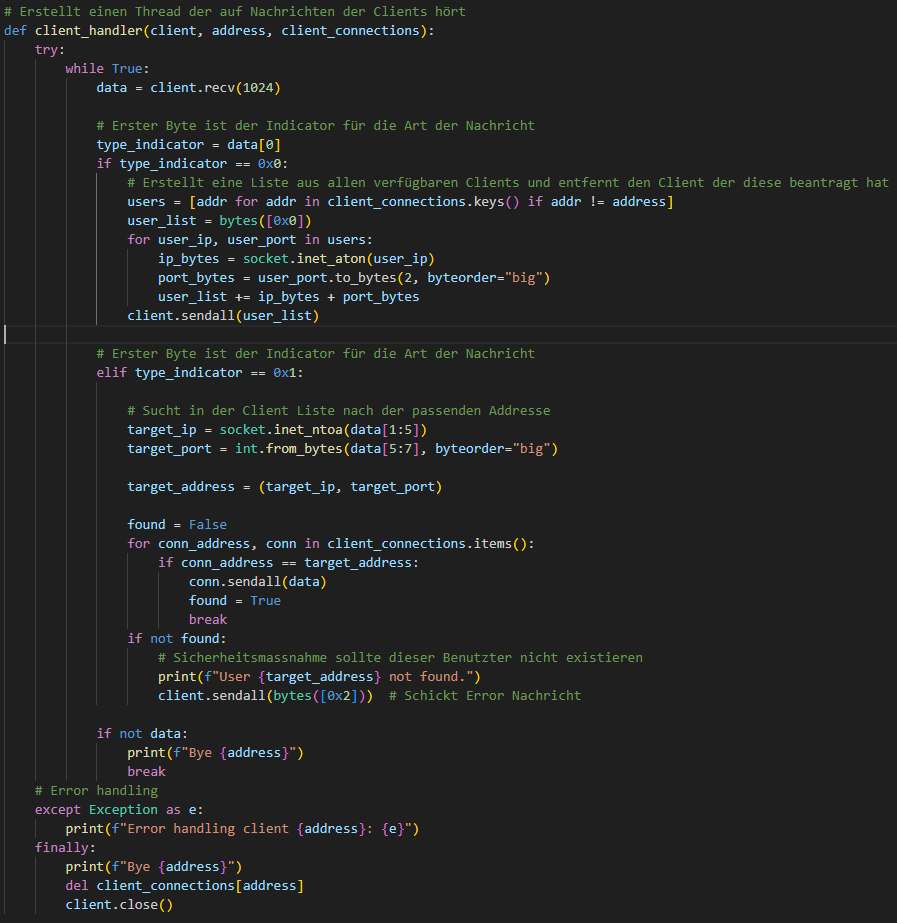
\includegraphics[width=0.6\linewidth]{picture-lib/Screenshot 2026-10-07 205030.png}
    \caption{Server.py Finale Version Abschnitt 2}
    \label{fig:A14}
\end{figure}

Beim Annehmen von Verbindungen hat sich wenig verändert. Es wurde lediglich die Puffergrösse von 4 KB ergänzt.

\begin{figure}[H]
    \centering
    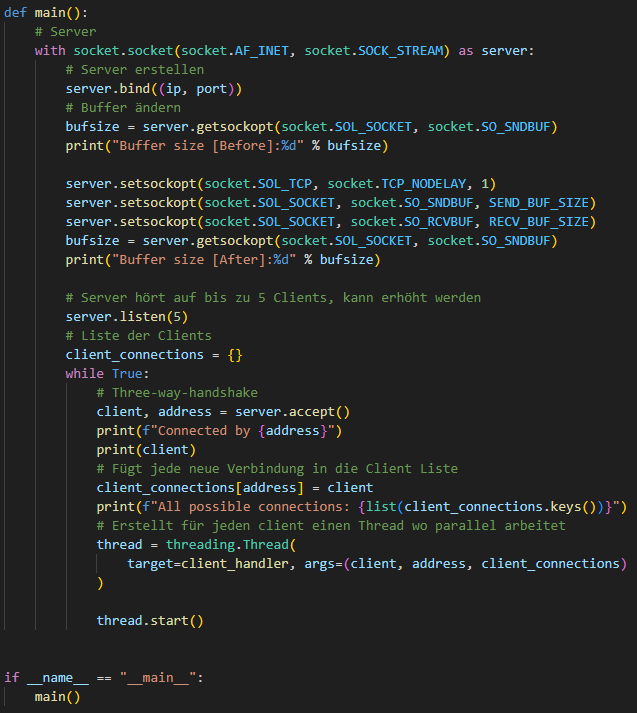
\includegraphics[width=0.5\linewidth]{picture-lib/Screenshot 2026-10-07 205047.png}
    \caption{Server.py Finale Version Abschnitt 3}
    \label{fig:A15}
\end{figure}

\subsection{Clientseite}

Hier werden Schlüssel und Variablen der Clientseite festgelegt. Wichtig ist, dass nur Benutzer mit demselben Schlüssel miteinander kommunizieren können. Der Schlüssel lässt sich jederzeit ändern, muss aber genau 16, 24 oder 32 Bytes lang sein. Ein längerer Schlüssel bietet mehr Sicherheit, verlängert aber das Ver- und Entschlüsseln leicht. Zudem müssen \texttt{exip} und \texttt{port} der IP-Adresse und dem Port des Servers entsprechen. Diese drei Werte müssen je nach Einsatz angepasst werden.

\begin{figure}[H]
    \centering
    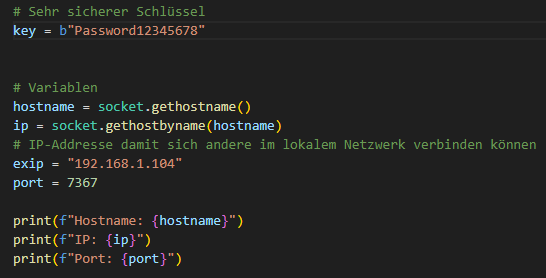
\includegraphics[width=0.5\linewidth]{picture-lib/Screenshot 2026-10-07 205128.png}
    \caption{Client.py Finale Version Abschnitt 1}
    \label{fig:A16}
\end{figure}

Die drei Funktionen aus \texttt{test.py} wurden übernommen. Zudem wurden kleinere Fehler in der Fehlerbehandlung und beim Port behoben.

\begin{figure}[H]
    \centering
    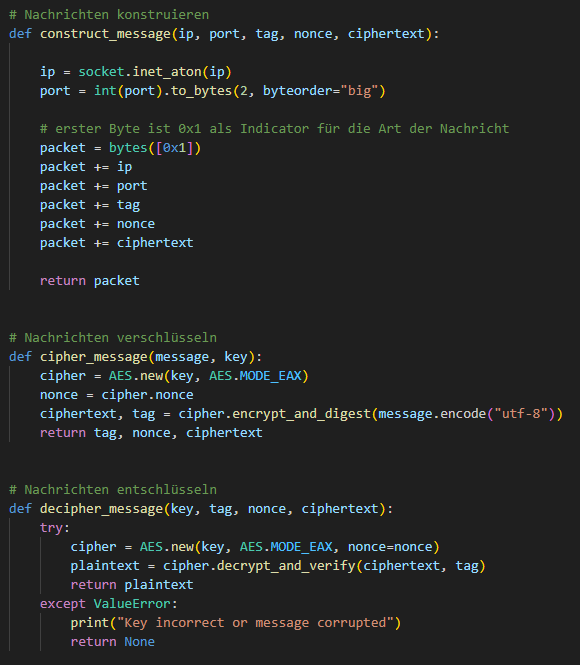
\includegraphics[width=0.5\linewidth]{picture-lib/Screenshot 2026-10-07 205225.png}
    \caption{Client.py Finale Version Abschnitt 2}
    \label{fig:A17}
\end{figure}

Auch das Empfangen von Daten musste wie auf der Serverseite stark angepasst werden. Zuerst wird geprüft, ob überhaupt Daten vorliegen, andernfalls wird der Vorgang abgebrochen. Danach wird zwischen drei Indikatoren unterschieden: Listenbefehl, Nachricht und Fehlercode.
Bei einer Nachricht mit dem Indikator 0x1 wird zuerst der Tag gelesen. Er umfasst 16 Byte ab dem achten Byte. Danach folgt der Nonce mit den nächsten 16 Byte, und alle übrigen Bytes gehören zur Nachricht. Sie wird mit \texttt{decipher\_message(\dots)} entschlüsselt und im Chatverlauf angezeigt.
Bei einer Liste mit dem Indikator 0x0 wird das erste Byte ignoriert und die Länge der übrigen Daten bestimmt. Sie werden in Blöcke von je 6 Byte aufgeteilt, wobei jeder Block die Informationen eines Benutzers enthält (IP-Adresse und Port). Diese Liste wird für die Combobox verwendet, in der der Benutzer den Empfänger auswählt. Standardmässig ist der erste Eintrag ausgewählt.
Trifft ein Fehlercode mit dem Indikator 0x2 ein, wird er im Terminal und im Chatverlauf angezeigt, damit der Benutzer weiss, dass der Empfänger nicht gefunden wurde.

\begin{figure}[H]
    \centering
    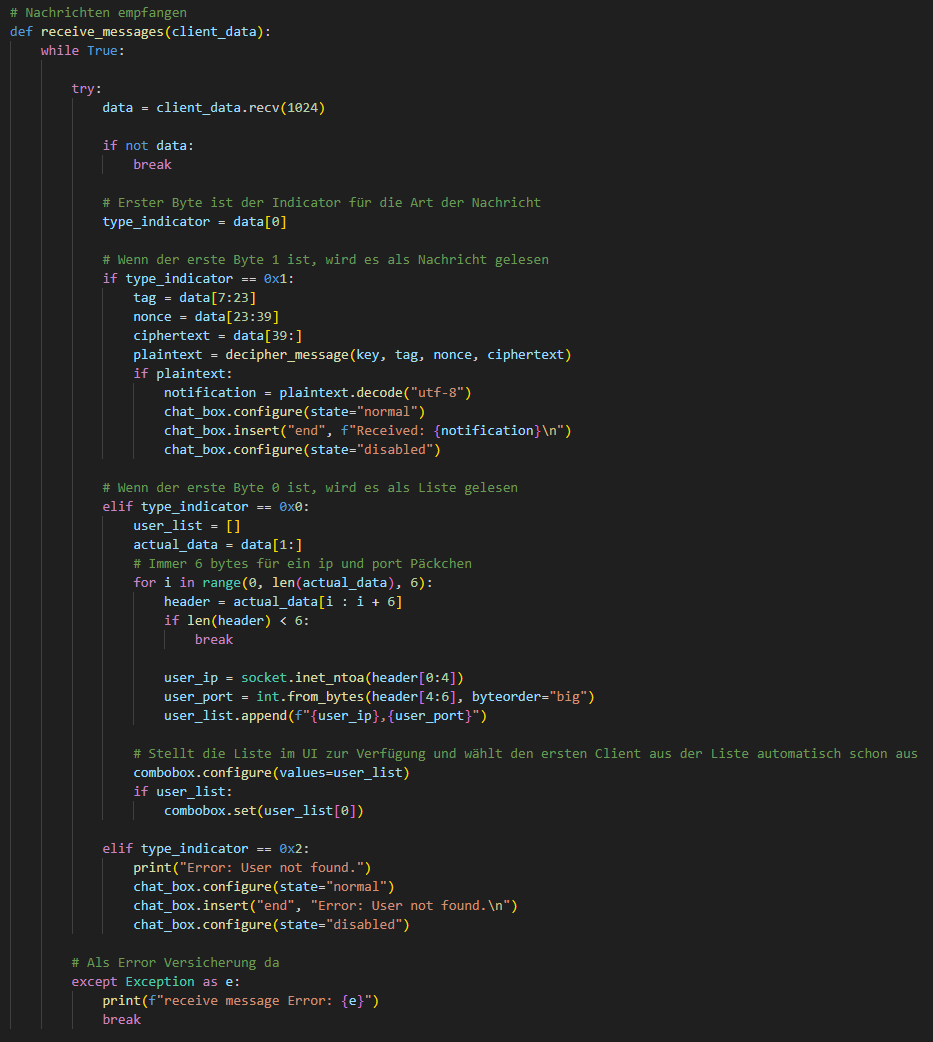
\includegraphics[width=0.75\linewidth]{picture-lib/Screenshot 2026-10-07 205237.png}
    \caption{Client.py Finale Version Abschnitt 3}
    \label{fig:A18}
\end{figure}

Die GUI wurde in einigen Punkten angepasst. Unter anderem wurde Tkinter durch die Bibliothek CustomTkinter erweitert. Sie ermöglicht ein moderneres Design mit abgerundeten Ecken und eine automatische Anpassung an das helle oder dunkle Farbschema des Computers. Weitere Einstellungen zur Anpassung sind in CustomTkinter standardmässig enthalten.

\begin{figure}[H]
    \centering
    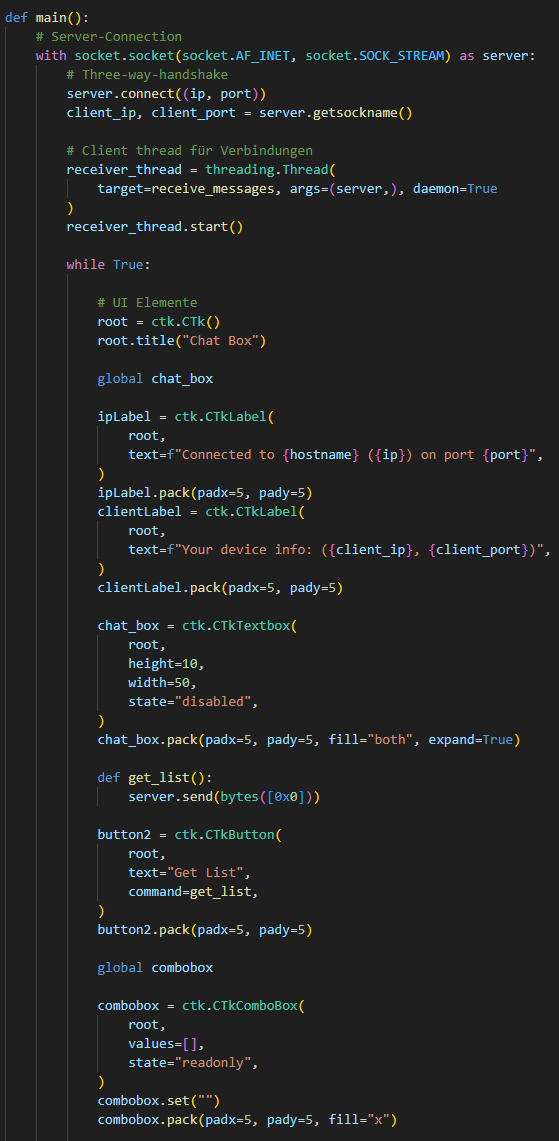
\includegraphics[width=0.5\linewidth]{picture-lib/Screenshot 2026-10-07 205316.png}
    \caption{Client.py Finale Version Abschnitt 4}
    \label{fig:A19}
\end{figure}

Die Funktion \texttt{send()} wurde ebenfalls an das Protokoll angepasst. Sie liest die benötigten Daten aus Eingabefeld und Combobox, konstruiert daraus ein Paket (\texttt{packet}) und sendet es.

\begin{figure}[H]
    \centering
    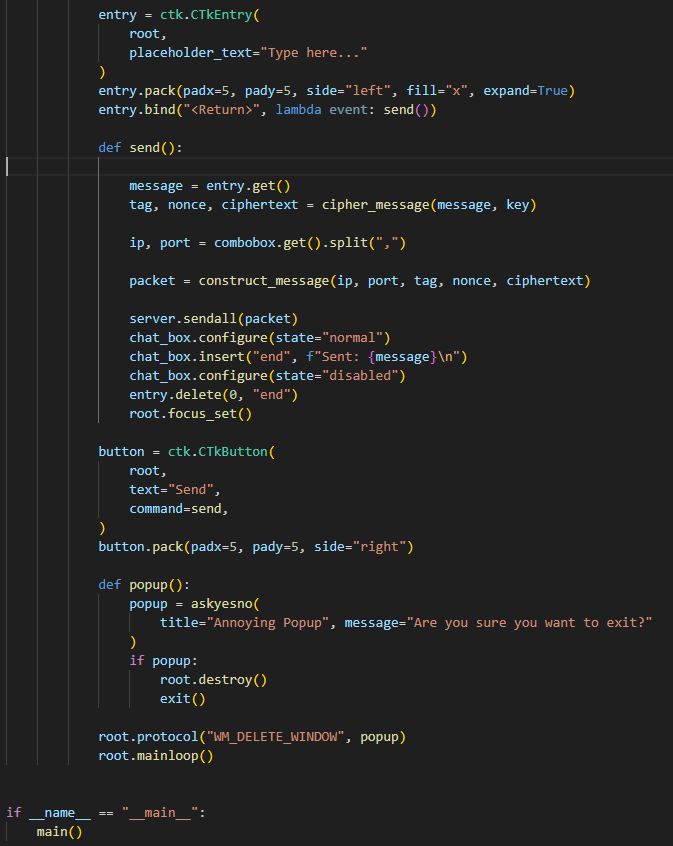
\includegraphics[width=0.5\linewidth]{picture-lib/Screenshot 2026-10-07 211314.png}
    \caption{Client.py Finale Version Abschnitt 5}
    \label{fig:A20}
\end{figure}

\subsection{Weitere Auswertungen}

Das fertige Produkt ist in Abbildung~\ref{fig:A21} zu sehen. Es zeigt den verbundenen Server sowie Informationen zur eigenen Chat Box und enthält alle Widgets, die für den Austausch einfacher Nachrichten nötig sind.

\begin{figure}[H]
    \centering
    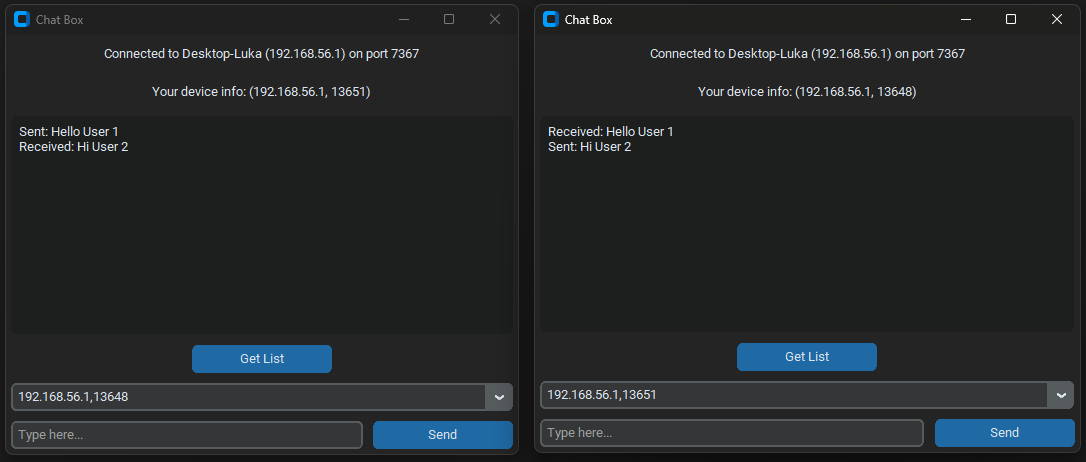
\includegraphics[width=0.75\linewidth]{picture-lib/Screenshot 2026-10-08 004928.png}
    \caption{Zwei Chat Boxen}
    \label{fig:A21}
\end{figure}

Beim Schliessen des Fensters erscheint die folgende Sicherheitsabfrage:

\begin{figure}[H]
    \centering
    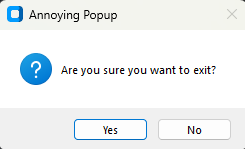
\includegraphics[width=0.5\linewidth]{picture-lib/Screenshot 2026-10-08 001339.png}
    \caption{Popup-Fenster}
    \label{fig:A22}
\end{figure}

Mit der Software Wireshark lassen sich Datenpakete in einem Netzwerk mitschneiden und auslesen.\citep{WiresharkOrg} Ich verglich eine Nachricht, die ohne Verschlüsselung gesendet wurde, mit einer verschlüsselten Nachricht. Der blau markierte Abschnitt ist in der unverschlüsselten Version (Abbildung \ref{fig:A23}) für jeden lesbar, der mit dem Netzwerk verbunden ist. In der verschlüsselten Version (Abbildung \ref{fig:A24}) besteht er nur aus Zeichen ohne erkennbaren Sinn. Erkennbar bleibt das erste Byte 01. Das ist beabsichtigt, denn es ist der Indikator [0x1], der eine Nachricht kennzeichnet. In Abbildung \ref{fig:A23} ist er nicht vorhanden.

Die Version ohne eigenes Protokoll benötigt mehr Platz für IP-Adresse und Port, da sie als umgewandelter String gesendet werden und nicht als rohe Bytes. Insgesamt benötigt die Version mit eigenem Protokoll jedoch mehr Bytes, da zusätzlich Tag und Nonce übertragen werden. Beide belegen unabhängig von der Länge der Nachricht je 16 Byte.

\begin{figure}[H]
    \centering
    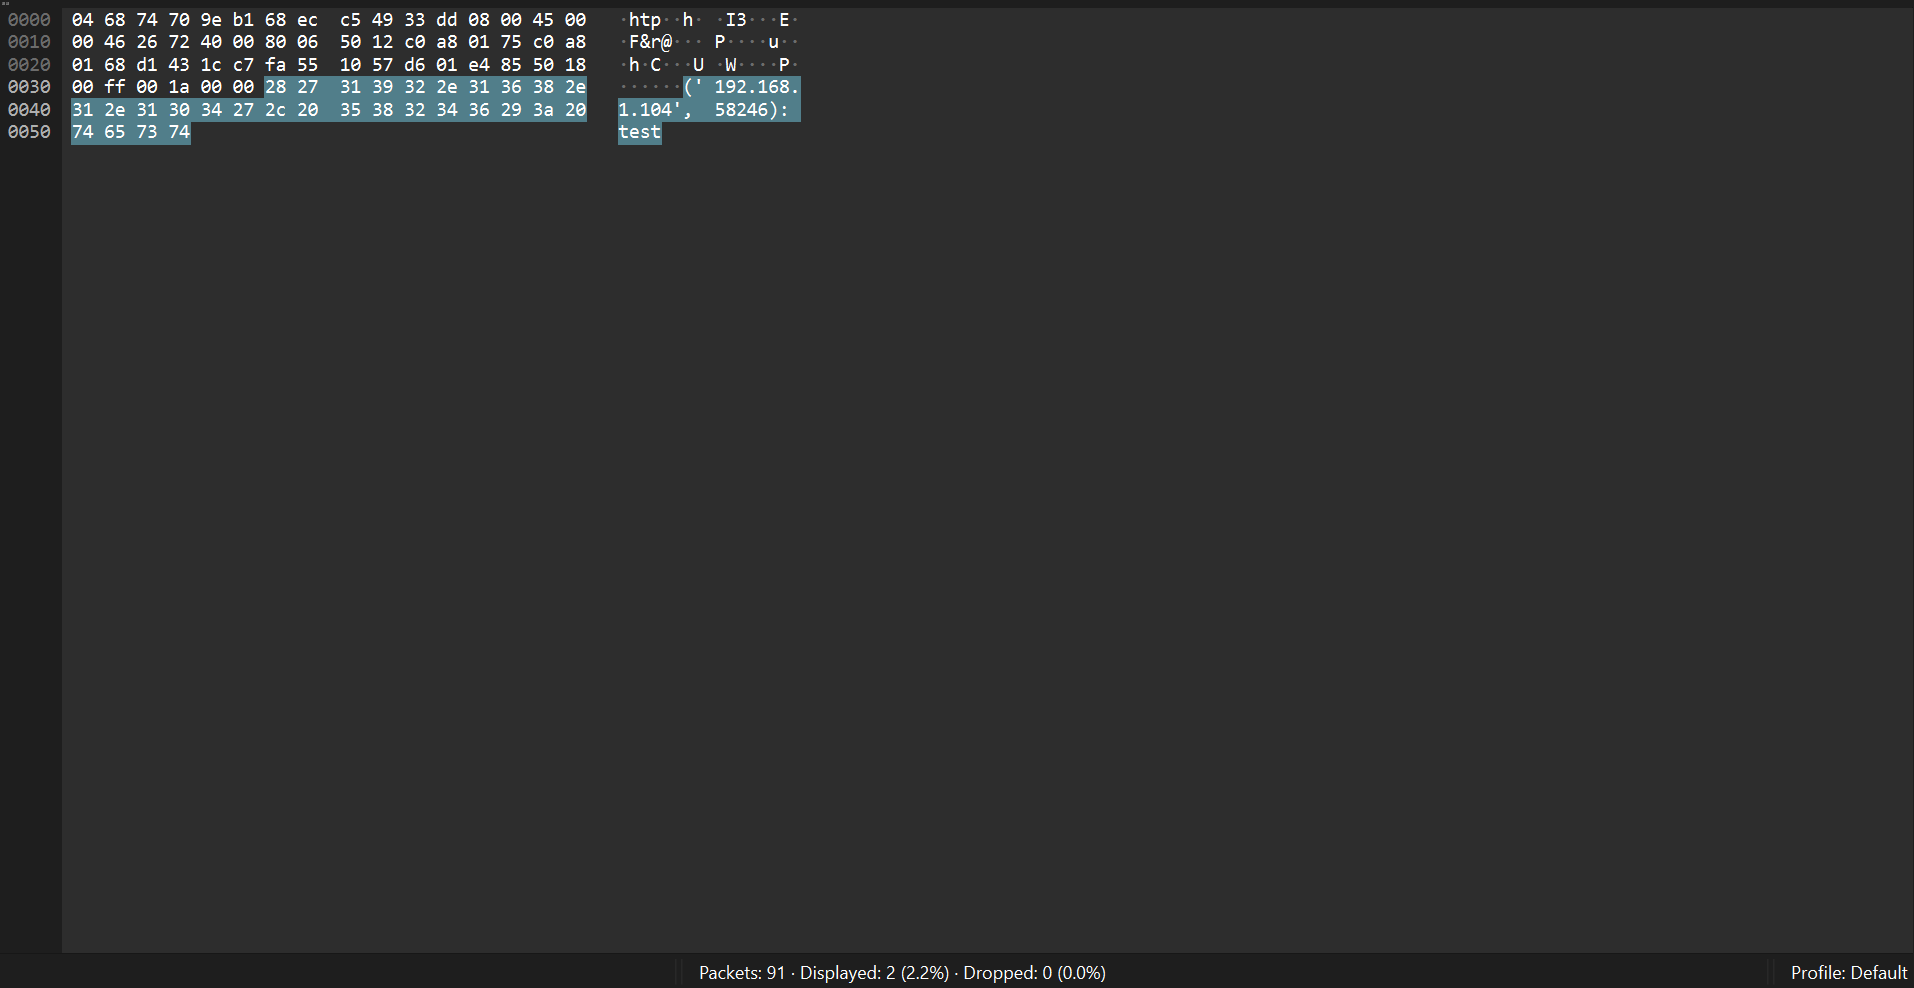
\includegraphics[width=1\linewidth]{picture-lib/Screenshot 2026-08-27 204201.png}
    \caption{Wireshark ohne Verschlüsselung und Protokoll}
    \label{fig:A23}
\end{figure}

\begin{figure}[H]
    \centering
    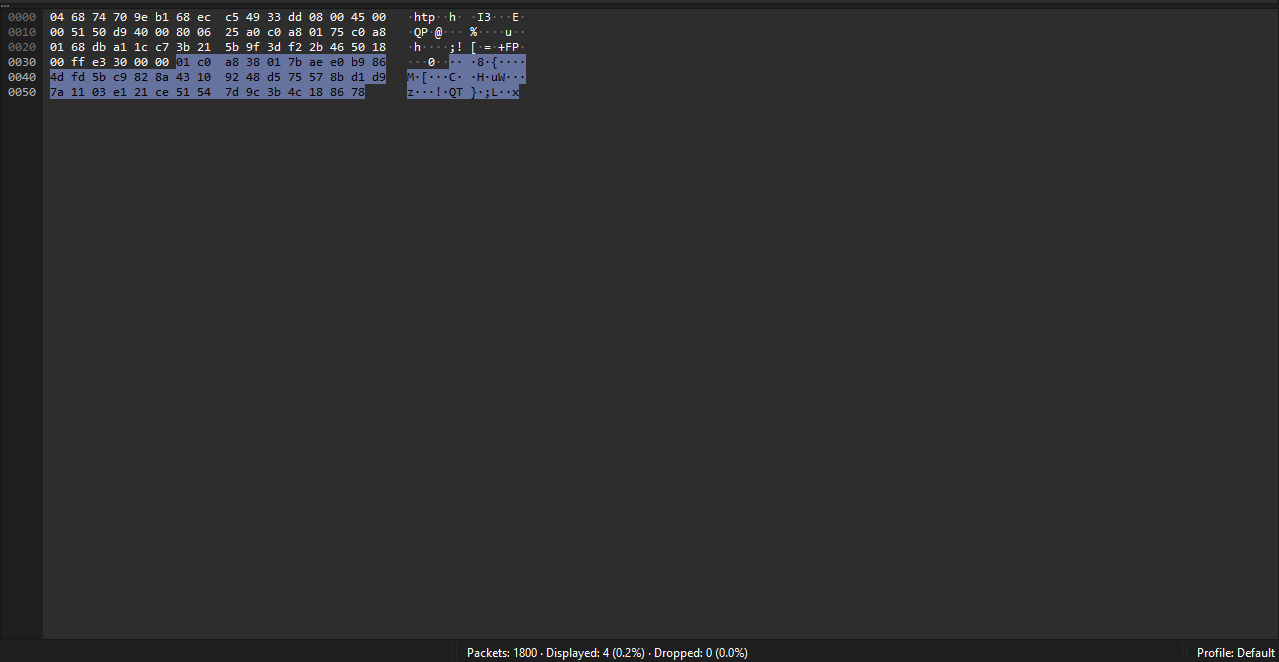
\includegraphics[width=1\linewidth]{picture-lib/Screenshot 2026-10-08 004141.png}
    \caption{Wireshark mit Verschlüsselung und Protokoll}
    \label{fig:A24}
\end{figure}

Der Inhalt der verschlüsselten Nachrichten ist mit Wireshark ohne Schlüssel nicht lesbar. Indikator, IP-Adresse und Port bleiben dagegen sichtbar, da der Server sie für die Zustellung auslesen muss. Der Verschlüsselungsvorgang beim Senden einer Nachricht ist so schnell, dass er im Betrieb nicht wahrnehmbar ist.
Die Bytes vor dem markierten Abschnitt gehören zu den Headern von TCP/IP. In beiden Abbildungen ist die erste Zeile gleich aufgebaut: \texttt{Ethernet II, Src: Intel\_XX:XX:XX (68:ec:c5:xx:xx:xx), Dst: CloudNetwork\_XX:XX:XX (04:68:74:xx:xx:xx)} beschreibt die zweite Schicht mit den MAC-Adressen von Sender und nächstem Empfänger. Sie bleiben gleich, solange dieselben Geräte miteinander kommunizieren, weil sie an die Hardware gebunden sind. Die zweite Zeile, \texttt{Internet Protocol Version 4, Src: 192.168.1.117, Dst: 192.168.1.104}, beschreibt die dritte Schicht mit den IP-Adressen. Die dritte Zeile, \texttt{Transmission Control Protocol, Src Port: 56225, Dst Port: 7367, Seq: 1, Ack: 1, Len: 41}, beschreibt TCP mit den Ports und der Länge der Nutzdaten in Bytes. Die Nutzdaten der Abbildung \ref{fig:A23} umfassen 30 Bytes, die der Abbildung \ref{fig:A24} 41 Bytes.